\documentclass[../Main.tex]{subfiles}

\begin{document}
\section{The Complex Plane}
We can identify $\C$ with $\R^2$, as seen in the previous chapter. We have the addition operation, which works as in $\R^2$:
\begin{equation*}
    z = z_1 + z_2 \iff (x, y) = (x_1 + x_2, y_1 + y_2)
\end{equation*}
But we also have multiplication:
\begin{equation*}
    z = z_1 z_2 \iff (x, y) = (x_1 x_2 - y_1 y_2, x_1 y_2 + x_2 y_1)
\end{equation*}
All of the above work in the normal way with $i^2 = -1$.

However, for many applications $\C$ is not enough. We require the extended complex plane, including the single point at infinity.
\begin{definition}{Extended complex plane}
    The \underline{extended complex plane} is defined as:
    \begin{equation*}
        \Cstar = \C \cup \{\infty\}
    \end{equation*}
    where the point $\infty$ is reached by going off in any direction on the plane and all directions are equivalent.
\end{definition}
This can be visualised using the Riemann Sphere. See figure~\ref{figRiemannSphere}.
\begin{figure}
    \centering
    \includegraphics[width=\linewidth]{Riemann sphere}
    \caption{Diagram of the Riemann Sphere}
    \label{figRiemannSphere}
\end{figure}
Any point $Z$ on the sphere is mapped onto $\C$ via the line from the top of the sphere through $Z$. The point at which it intersects the plane $w = 0$ is $z \in \C$. The single point at infinity is identified with $Z = (0, 0, 1)$.
\section{Complex Differentiation}
\begin{definition}{Differentiability}
    A function $f : \C \mapsto \C$ is \underline{differentiable} at $z \in \C$ if:
    \begin{equation*}
        f'(z) = \lim_{\delta z \to 0} \frac{f(z + \delta z) - f(z)}{\delta z}
    \end{equation*}
    exists and is independent of the direction of approach.
\end{definition}
\begin{remark}
    Being independent of the direction of approach is very restrictive!
\end{remark}
\begin{definition}{Neighbourhood}
    A \underline{neighbourhood} $V$ around a point $z \in \C$ is a set for which there exists $r > 0$ such that the ball $B_r(z) = \subsetselect{w \in \C}{|w - z| < r}$ is contained within $V$.
\end{definition}
\begin{remark}
    We can understand a neighbourhood as a set that allows for movement a small (but non-zero) distance in any direction from the point $z$.
\end{remark}
\begin{definition}{Analytic function}
    A function $f : \C \mapsto \C$ is \underline{analytic} at a point $z$ if there exists a neighbourhood of $z$ for which $f'(z)$ exists.
\end{definition}
\begin{definition}{Entire}
    A function $f : \C \mapsto \C$ is \underline{entire} if it is analytic throughout $\C$.
\end{definition}
\begin{remarks}
    \item If a function is analytic around a point, it is infinitely differentiable there [not proven in this course]
    \item A bounded, entire function must be constant [to be proved later].
\end{remarks}
Consider functions of the form:
\begin{align*}
    f : \C &\mapsto \C\\
    x + i y &\mapsto u(x, y) + i v(x, y)
\end{align*}
where $u, v : \R^2 \mapsto \R$.

Suppose that $f$ is differentiable at $z = x + iy$. Then we can take $\delta z$ in any direction we like. Take $\delta z = \delta x$:
\begin{align*}
    f'(z) &= \lim_{\delta x \to 0} \frac{f(z + \delta x)-f(x)}{\delta x} \\
    &= \lim_{\delta x \to 0} \frac{i(x + \delta x, y) + i v(x + \delta x, y) - u(x, y) - iv(x, y)}{\delta x} \\
    &= \frac{\partial u}{\partial x} + i \frac{\partial v}{\partial x}
\end{align*}
Now instead taking $\delta z = i\delta y$:
\begin{align*}
    f'(z) &= \lim_{\delta y \to 0} \frac{f(z + i \delta y) - f(z)}{i\delta y} \\
    &= \lim_{\delta y \to 0} \frac{u(x, y + \delta y) + i v(x, y + \delta y) - u(x, y) - iv(x, y)}{i \delta y} \\
    &= \frac{\partial v}{\partial y} - i \frac{\partial u}{\partial y}
\end{align*}
And so for differentiability we require:
\begin{equation*}
    \frac{\partial u}{\partial x} + i \frac{\partial v}{\partial x} = \frac{\partial v}{\partial y} - i \frac{\partial u}{\partial y}
\end{equation*}
\begin{proposition}[Cauchy-Riemann Identities]
    A differentiable function $f = u + i v$ satisfies the Cauchy-Riemann identities:
    \begin{equation}
        \frac{\partial u}{\partial x} = \frac{\partial v}{\partial y}\qquad\frac{\partial v}{\partial x} = -\frac{\partial u}{\partial y}
        \label{eqnCRIds}
    \end{equation}
    \label{propCRIds}
\end{proposition}
\begin{proposition}
    If $f = u + iv$ satisfies \eqnref{eqnCRIds} at $z = z_0$, and the partial derivatives are continuous in a neighbourhood around $z$, then $f$ is differentiable at $z_0$.
    \label{propCRIdsConverse}
\end{proposition}
\begin{proof}
    See the course IB Complex Analysis.
\end{proof}
\begin{propositions}{
        Suppose that $f$ and $g$ are differentiable complex functions.
        \label{propsComplexDiffRules}
    }
    \item $\frac{d}{dz} (f(z) g(z)) = f'(x) g(x) + f(x) g'(x)$ \label{propProductRule}
    \item $\frac{d}{dx}(f \circ g)(z) = f'(g(z)) g'(z)$ \label{propChainRule}
\end{propositions}
\begin{proof}
    Define:
    \begin{align*}
        \varpi &= \frac{f(z + h) - f(z)}{h} - f'(z) \implies f(z + h) = f(z) + h (\varpi + f') \\
        \overline{\varpi} &= \frac{g(z + h) - g(z)}{h} - g'(z) \implies g(z + h) = g(z) + h (\overline{\varpi} + g')
    \end{align*}
    By definition, $\lim_{h \to 0} \varpi = \lim_{h \to 0} \overline{\varpi} = 0$.
    \begin{align*}
        \frac{d}{dz} f(z) g(z) &= \lim_{h \to 0} \frac{f(z + h) g(z + h) - f(z) g(z)}{h} \\
        &= \lim_{h \to 0} \frac{\left[f(z) + h \varpi + hf'(z)\right] \left[g(z) + h \overline{\varpi} + h g'(z)\right]}{h} \\
        &= \lim_{h \to 0}\left(\frac{f(z) (\overline{\varpi} + g'(z))h + h(\varpi + f'(z))g(z)}{h} + O(h)\right) \\
        &= f'(z) g(z) + f(z) g'(z)
    \end{align*}
    To prove the chain rule, we change the notation for $\varpi$ and $\overline{\varpi}$ as follows:
    \begin{align*}
        \varpi[z, h] &= \frac{f(z + h) - f(z)}{h} \\
        \overline{\varpi}[z, h] &= \frac{g(z + h) - g(z)}{h}
    \end{align*}
    Then:
    \begin{align*}
        \frac{d}{dz}&f(g(z))= \lim_{h \to 0} \frac{f(g(z + h)) - f(g(z))}{h} \\
        &= \lim_{h \to 0} \frac{f(g(z) + h (\overline{\varpi}[z, h] + g'(z))) - f(g(z))}{h} \\
        &= \lim_{h \to 0} \frac{h(\overline{\varpi}[z, h] + g'(z))(\varpi[g(z), h(\overline{\varpi}[z, h] + g'(z))] + f'(g(z)))}{h} \\
        &= \lim_{h \to 0} (\overline{\varpi}[z, h] + g'(z))(\varpi[g(z), h(\overline{\varpi}[z, h] + g'(z))] + f'(g(z))) \\
        &= \lim_{h \to 0}\left\{ \overline{\varpi}[z, h]\varpi[g(z), h(\overline{\varpi}[z, h] + g'(z))] + \overline{\varpi}[z, h]f'(g(z))\right.\\
        &\qquad\left.+ g'(z)\varpi[g(z), h(\overline{\varpi}[z, h] + g'(z))] + f'(g(z))g'(z)\right\}\\
        &= f'(g(z))g'(z)
    \end{align*}
    since this is the only term without $\varpi$ or $\overline{\varpi}$.
\end{proof}
In Ex1, we find that analyticity implies that:
\begin{equation*}
    \text{$f$ analytic} \iff \frac{\partial f}{\partial \overline{z}}
\end{equation*}
Such functions are also called holomorphic.
\begin{examples}[Examples of analytic functions]{
        Consider the following functions.
        \label{exAnalyticFuncs}
    }
    \item $f(z) = z$. Then we check \eqnref{eqnCRIds}:
        \begin{align*}
            \frac{\partial u}{\partial x} &= 1 & \frac{\partial v}{\partial y} &= 1 \\
            \frac{\partial u}{\partial y} &= 0 & -\frac{\partial u}{\partial y} &= 0 \\
        \end{align*}
    \item $f(z) = e^z = e^x(\cos(y) + i\sin(y))$.
        \begin{align*}
            \frac{\partial u}{\partial x} &= e^x\cos(y) & \frac{\partial v}{\partial y} &= e^x \cos(y) \\
            \frac{\partial u}{\partial y} &= -e^x \sin(y) & -\frac{\partial u}{\partial y} &= -e^x\sin(y) \\
        \end{align*}
    \item $f(z) = z^m$ follows from induction, with $f'(z) = mz^{m-1}$. Note that a linear combination of analytic functions is still analytic. With this, we see that polynomials are analytic.
    \item $f(z) = \frac1z = \frac{x - iy}{x^2 + y^2}$.
        \begin{align*}
            \frac{\partial u}{\partial x} &= \frac{y^2 - x^2}{(x^2 + y^2)^2} = \frac{\partial v}{\partial y} \\
            \frac{\partial v}{\partial x} &= \frac{2xy}{(x^2 + y^2)^2} = -\frac{\partial u}{\partial y}
        \end{align*}
        However, at the origin this fails.
\end{examples}
\begin{examples}[Examples of non-analytic functions]{
        Consider the following functions.
    }
    \item $f(z) = \Re(z)$
        Here $u(x, y) = x, v(x, y) = 0$. Therefore,
        \begin{equation*}
            \frac{\partial u}{\partial x} = 1,\quad \frac{\partial v}{\partial y} = 0
        \end{equation*}
        which violates \eqnref{eqnCRIds}.
    \item $f(z) = |z|$ Here we have the same problem as last time, where $v = 0$ and $u \neq 0$. However, at $z = 0$ \eqnref{eqnCRIds} is satisfied. This is still not analytic because we require that this is satisfied in a neighbourhood around a point, which is not the case.
    \item $f(z) = \overline{z}$
        Here $u(x, y) = x, v(x, y) = -y$. Therefore,
        \begin{equation*}
            \frac{\partial u}{\partial x} = 1,\quad \frac{\partial v}{\partial y} = -1
        \end{equation*}
        which violates \eqnref{eqnCRIds}.
\end{examples}
\section{Harmonic Functions}
\begin{definition}{Harmonic conjugate}
    Two functions $u, v : \R^2 \mapsto \R$ satisfying equation~\ref{eqnCRIds} (Cauchy-Riemann Equations) are called \underline{harmonic conjugates}.
\end{definition}
If we know either $u$ or $v$, we can find the other up to a constant.
\begin{example}
    Take $u(x, y) = x^2 - y^2$. Then we have:
    \begin{align*}
        \frac{\partial v}{\partial y} &= 2x \implies 2xy + \hat{v}(x) \\
        \frac{\partial v}{\partial u} &= 2y \implies \hat{v}'(x) = 0
    \end{align*}
    Therefore $v = 2xy + \alpha$ where $\alpha \in \R$ is a constant.

    Now our complex-valued function $f$ is given by:
    \begin{align*}
        f(x + iy) &= x^2 - y^2 + 2iyx + i\alpha \\
        &= (x + iy)^2 + i\alpha \\
        &= z^2 + i\alpha
    \end{align*}
    Then this is analytic because it depends only on $z$ and not $\bar{z}$.
\end{example}
\begin{definition}{Harmonic function}
    A function $f(x, y) : \R^2 \mapsto \R$ is \underline{harmonic} if it satisfies the \underline{Laplace equation}:
    \begin{equation}
        \Delta f = \left(\frac{\partial^{2}}{\partial x^{2}} + \frac{\partial^{2}}{\partial y^{2}}\right) f = 0
        \label{eqnLaplace}
    \end{equation}
\end{definition}
\begin{proposition}
    The real and imaginary parts of an analytic function are harmonic.
    \label{propAnaGivesHrm}
\end{proposition}
\begin{proof}
    Let $f = u + iv$, as in the above. Let $f$ be analytic, so we can use equation~\ref{eqnCRIds}:
    \begin{align*}
        \frac{\partial^{2}u}{\partial x^{2}} &= \frac{\partial}{\partial x} \left(\frac{\partial v}{\partial y}\right) \\
        &= \frac{\partial}{\partial y} \left(\frac{\partial v}{\partial x}\right) \\
        &= \frac{\partial}{\partial y} \left(-\frac{\partial u}{\partial y}\right) = -\frac{\partial^{2}u}{\partial y^{2}}.
    \end{align*}
    Therefore $\Delta u = 0$. The same applies for $v$.
\end{proof}
\section{Multivalued Functions}
In this section, we study multivalued functions and use the example of $\log(z)$ throughout.

For $z = re^{i\theta}$, we define $\log(z) = \log(r) + i\theta$. However, $\theta$ can take infinitely many values to give the same $z$.

As an example, $\log(i)$ takes many values: $i \frac{\pi}{2}, \frac{5\pi}{2} i, \cdots$. Therefore, $\log$ has to be multivalued. In principle this it fine, but we must be careful (and consistent).

\begin{figure}
    \centering
    \begin{tikzpicture}[scale=1]
        \draw[->] (-5, 0) -- (5, 0) node[right] {$\Re$};
        \draw[->] (0, -3) -- (0, 5) node[above] {$\Im$};
        \begin{scope}[every node/.style={fill, circle, minimum size=2mm, inner sep=0pt}]
            \node at (3, 3) (Z1) [label=below left:$z_1$] {};
            \node at (-3, 0) (Z2) [label=below right:$z_2$] {};
            \node at (0, 0) (Z3) [label=below left:$0$] {};
        \end{scope}
        \draw (Z1) circle[radius=1.75];
        \draw ($(Z1) + (1.5, 1.5)$) node{$C_1$};
        \draw (Z2) circle[radius=1.5];
        \draw ($(Z2) + (0, 1.7)$) node{$C_2$};
        \draw (Z3) circle[radius=1];
        \draw ($(Z3) + (1, -0.7)$) node{$C_3$};
    \end{tikzpicture}
    \caption{Diagram of $\log$, with different circles}
    \label{figLogPlot}
\end{figure}

Consider figure~\ref{figLogPlot}. We see that, on $C_1$, $\arg(x) \in \left(0, \frac\pi2\right)$, and so $\log$ is single valued here. Similarly, $\arg(z)$ takes values $\left(\frac\pi2, \frac{3\pi}{2}\right)$ on $C_3$, so again $\log$ is single-valued.

A problem arises with $C_3$. We find that, as we go around the circle, $\arg(z)$ keeps increasing and so does $\Im(\log(z))$, so $\log$ is multivalued on this circle.

\subsection{Branch Points}
\begin{definition}{Branch point}
    A \underline{branch point} of a function $f : \C \mapsto \C$ is a point $z_0$ such that no closed curve $C$ contained in an arbitrarily small neighbourhood around $z_0$ and encircling $z_0$ exists such that $f$ is single valued and continuous on $C$.
\end{definition}
\begin{examples}{
        
    }
    \item $f(z) = \log(z - a)$ for $a \in \C$ has a branch point at $a$. We see this by taking a circle $|z - a| = r$, and evaluating log there.
    \item Consider $f(z) = z^\alpha$, where $\alpha \in \R \backslash \Z$. Then $f(z) = r^\alpha r^{i \alpha \theta}$ along a circle of radius $r$ around $z = 0$.
        \begin{itemize}
            \item $\theta = 0 \implies f(z) = r^\alpha$
            \item $\theta = 2\pi \implies f(z) = r^\alpha e^{2 \pi i \alpha} \neq r^\alpha$.
        \end{itemize}
        So we have a branch point at $z = 0$. In $\Cstar$, there is a branch point at $\infty$. We know this by considering $f(\frac1\xi)$, and this also has a branch point at $\xi = 0$.
    \item $f(z) = \log\left(\frac{z-1}{z+1}\right) = \log(z-1) - \log(z+1)$. By the first example we must have at least two branch points, at $z = \pm 1$.
    \item We have another branch point of $\log$ on $\Cstar$. We can see this easily by taking $g(\xi) = f(\frac1\xi) = -\log(\xi)$, and we know this has a branch point at $0$. What about the third function, $f(z) = \log\left(\frac{z-1}{z+1}\right)$? Change variable:
        \begin{align*}
            f\left(\frac1\xi\right) &= \log\left(\frac{1 - \xi}{1 + \xi}\right) \\
            &= -2\xi + O(\xi)^2
        \end{align*}
        Which behaves nicely as $\xi \to 0$.
\end{examples}
\subsection{Branch Cuts}
If we wish to make $\log(z)$ continuous and single-valued, we must forbid any curve from encircling the origin (where the branch point is). We do this by drawing a boundary curve that the function may not cross.
\begin{definition}{Branch cut}
    A \underline{branch cut} is a curve that connects two branch points. Curves on which the function is defined may not cross the branch cut.
\end{definition}
Continuing the example of $\log(z) = \log(|z|) + i \arg(z)$, we can take the branch cut along the negative real axis. This is permissible because it connects $z = 0$ with $z = \infty$.

Now $\log$ is continuous, single-valued and differentiable on any curve that does not cross the cut. Its derivative is:
\begin{equation*}
    \frac{d}{dz} \log(z) = \frac1z
\end{equation*}
\begin{definition}{Branch}
    For a multivalued function $f$ defined on $\Cstar$ with a branch cut, the \underline{branch} of the function is the value of $f$ assigned to the domain that remains.
\end{definition}
\begin{examples}{
        We have different ways to denote the function's branch and branch cut.
    }
    \item $\log(z) = \log(|z|) + i \arg(z),\quad \arg \in (-\pi, \pi)$.
        Then this defines the branch cut (along $\arg(z) = \pi$) and the branch (by giving a range of values of $\arg$).
    \item We can specify the branch cut, and give the value of the function at a point not on the cut.
    \item \textbf{Non-Examinable:} Riemann Surfaces. Riemann imagined something more clever than this abrupt jump. Instead, consider the branches as different copies of $\Cstar$ and ``glue them together'' along the branch cuts. See figure~\ref{figRiemannSurface}.
\end{examples}
\begin{figure}
    \centering
    \includegraphics[width=\linewidth]{Riemann surfaces}
    \caption{Image of the Riemann surfaces of $\log$}
    \label{figRiemannSurface}
\end{figure}
So far we have mostly considered branch points at $z = 0$ and $z = \infty$. We would also like to be able to deal with cases with branch points at different places, and more than 2 branch points.
\begin{figure}
    \centering
    \begin{tikzpicture}[scale=1]
    \draw[->] (-3, 0) -- (5, 0) node[right] {$\Re$};
    \draw[->] (0, -3) -- (0, 3) node[above] {$\Im$};
    
    \draw[branchcut] (-3, 0) -- (0, 0);
    \draw[branchcut] (1.5, 0) -- (5, 0);

    \begin{scope}[every node/.style={fill, circle, minimum size=2mm, inner sep=0pt}]
        \node at (1.5, 0) [label=below left:$z_1$] {};
        \node at (0, 0) [label=below left:$0$] {};
    \end{scope}

    \end{tikzpicture}
    \caption{Branch cut for a function with 3 branch points}
    \label{figThreePointBranchCuts}
\end{figure}
\begin{example}
    Consider $f(z) = [z(z-1)]^{\frac13}$. We suspect that there are branch points at $z \in \{0, 1, \infty\}$. Indeed, we can check that this is true. We can define a branch cut to be the lines from $z=0$ along $\arg(z) = \pi$, and from $z = 1$ along $\arg(z) = 0$. See figure~\ref{figThreePointBranchCuts}.

    In order to define the branch, we consider $z_0 = re^{i \theta}$ and $z_1 = 1 + r_1 e^{i\theta_1}$. Therefore,
    \begin{equation*}
        f(z) = (r r_1)^{\frac12} e^{\frac{i(\theta + \theta_1)}{3}}, \theta \in (-\pi, \pi], \theta_1 \in [0, 2\pi)
    \end{equation*}
    Then to change the branch, we would change the ranges of $\theta$ and $\theta_1$.
\end{example}
\begin{example}
    Return to the example of:
    \begin{equation*}
        f(z) = \log\left(\frac{z-1}{z+1}\right)
    \end{equation*}
    We saw that $f$ has branch points at $z = \pm 1$. We can check, also, that it does not have a branch point at $z = \infty$. We then can consider two different branch cuts:
    \begin{itemize}
        \item The simplest branch cut, connecting $z = \pm 1$ with a straight line (through the origin)
        \item A more complex branch cut, connecting $z = \pm 1$ with an infinite line through $z = \infty$, going the opposite way around the Riemann sphere. Note this is absolutely fine because we are \textit{passing through} the single point at infinity, not connecting to it as we have done previously (using half-lines).
    \end{itemize}
    We will take the first option. We define the branch using:
    \begin{equation*}
        z_0 = re^{i\theta},\quad z_1 = r_1 e^{i\theta_1}
    \end{equation*}
    Then we have the function $f$ defined:
    \begin{equation*}
        f(z) = \log\left(\frac{r_1}{r}\right) + i(\theta_1 - \theta)
    \end{equation*}
    where $r$ and $r_1$ are defined in terms of $\theta$ and $\theta_1$.

    But what ranges should we permit for $\theta$ and $\theta_1$?
    We must choose the same range for both, in order for the discontinuity in both $\theta$ and $\theta_1$ to cancel on the half-line $\arg(z-1) = 0$. Choose $\theta, \theta_1 \in [0, 2\pi)$.
\end{example}
\begin{definition}{Complete Branch Cut}
    Let $f(z)$ have branch points $z_1, z_2, \cdots$. A \underline{complete branch cut} of $f$ is a set of cuts with:
    \begin{enumerate}
        \item every branch point has a branch cut ending on it;
        \item both ends of a branch cut end on a branch point.
    \end{enumerate}
\end{definition}
\section{\moeb Maps}
\begin{definition}{\moeb map}
    A \underline{\moeb map} is a map:
    \begin{align*}
        \mu : \C &\mapsto \C\\
        z &\mapsto \frac{az + b}{cz + d}
    \end{align*}
    with $a, b, c, d \in \C$ with $ad \neq bc$.
\end{definition}
\begin{remarks}
    \item If $ad = bc$, then $\mu$ maps $\C$ to a single point;
    \item $\mu$ is analytic except for when $z = -\frac{d}{c}$.
    \item Extending $\mu$ to $\Cstar \mapsto \Cstar$, $\mu$ is invertible with:
        \begin{align*}
            \mu^{-1} : \Cstar &\mapsto \Cstar\\
            z &\mapsto \frac{-dz + b}{cz - a}
        \end{align*}
\end{remarks}
\begin{definition}{Circline}
    A \underline{circline} is either a line or a circle on $\C$. On the Riemann sphere, this is a circle. It becomes a line on $\C$ if the circle passes through $\infty$.
\end{definition}
A \underline{Circle of Apollonius} is defined by:
\begin{equation*}
    \abs{z - z_1} = \lambda \abs{z - z_2} \text{ where } z_1 \neq z_2, \lambda \in \R^+
\end{equation*}
\begin{proposition}
    Let $\mu$ be a \moeb map. Then $\mu$ maps circlines to circlines.
    \label{propMobCirclines}
\end{proposition}
\begin{proof}
    A circline obeys:
    \begin{equation*}
        \abs{z - z_1} = \lambda \abs{z - z_2}
    \end{equation*}
    Then let $w = \mu(z)$.
    \begin{align*}
        \abs{-\frac{-dw + b}{cw - a} - z_1}&= \lambda \abs{\frac{-dw + b}{cw - a} - z_2} \\
        \intertext{Multiply by $\abs{cw - a}$:}
        \abs{-dw + b - z_1 (cw - a)} &= \lambda \abs{-dw + b - z_2(cw - a)} \\
        \abs{-(d - c z_1)w + b + z_1 a} &= \lambda \abs{-(d + c z_2)w + b + a z_2} \\
        \abs{w - \frac{b + z_1 a}{d + c z_1}} &= \lambda \frac{\abs{d + c z_2}}{\abs{c + d z_1}} \abs{w - \frac{b + a z_2}{d + c z_2}}
    \end{align*}
    Therefore we have found the required form $\abs{w - w_1} = \lambda^\star \abs{w - w_2}$.
    $w_1 = \mu(z_1)$ and $w_2 = \mu(z_2)$. $\lambda^\star$ has a less nice form:
    \begin{equation*}
        \lambda^\star = \frac{\abs{c + d z_1}}{\abs{c + d z_2}} \lambda.
    \end{equation*}
\end{proof}
Geometrically, we need 3 points in $\Cstar$ to define a circline.
\begin{proposition}
    Let $\alpha, \beta, \gamma$ be distinct points in $\C$. Let also $\tilde{\alpha}, \tilde{\beta}, \tilde{\gamma}$ be distinct point in $\C$. Then there exists a \moeb map that sends:
    \begin{align*}
        \alpha &\mapsto \tilde{\alpha} \\
        \beta &\mapsto \tilde{\beta} \\
        \gamma &\mapsto \tilde{\gamma}
    \end{align*}
    \label{propMobThreePoint}
\end{proposition}
\begin{proof}
    Consider the map:
    \begin{equation*}
        \mu_{z_1, z_2, z_3}(z) = \frac{z_2 - z_3}{z_2 - z_1} \frac{z - z_1}{z - z_3}
    \end{equation*}
    Then this sends:
    \begin{align*}
        z_1 &\mapsto 0 \\
        z_2 &\mapsto 1 \\
        z_3 &\mapsto \infty
    \end{align*}
    Therefore, the composition required is:
    \begin{equation*}
        \mu = \mu_{\tilde{\alpha}, \tilde{\beta}, \tilde{\gamma}}^{-1} \circ \mu_{\alpha, \beta, \gamma}
    \end{equation*}
\end{proof}
\section{Conformal Mappings}
We would like to see how analytic functions map act on subsets of $\C$. We will give examples first to gain intuition, then we will formalise our notions.
\begin{example}
    Consider $f(z) = z^2$. By considering $z = re^{i\theta}$, we see that $f$ doubles the argument $\theta \mapsto 2\theta$, and stretches or squishes based on $|z|$, $r \mapsto r^2$.
    \label{expSquare}
\end{example}
\begin{example}
    Let $f(z) = e^z$. By considering $z = x + iy$, we see $f(z) = e^x e^{iy}$.

    Therefore, the real part of $z$ determines the radius of $f(z)$, and the imaginary part determines the argument of $f(z)$.

    Horizontal lines, $y = c$, map to lines of fixed $\theta$. Vertical lines, $x = c$, map to circle segments.

    Therefore, a rectangle in $\C$ maps to a segment of an annulus under $f$.
    \label{expExp}
\end{example}
\begin{definition}{Conformal map}
    A \underline{conformal map} is a map $f : U \mapsto V$ between two open sets $U, V \subseteq C$ which is analytic and whose derivative $f'$ is non-zero throughout.
\end{definition}
\begin{remark}
    Often, we require that the map is a bijection.
\end{remark}
\begin{proposition}
    A conformal map preserves the magnitude of angles between intersecting lines.
    \label{propConfMapPreserveAngles}
\end{proposition}
\begin{proof}
    Let $z_1(t)$ be a curve in $\C$ with $z_0 = z_1(t_0)$. The curve $z_1(t)$ at $t = t_0$ makes an angle $\theta$ with the horizontal. $\theta = \arg(z_1'(t_0))$.

    Let $f$ be a conformal map such that $\xi_1(t)$ is the image of $z_1(t)$ under $f$. Then the angle between this and the horizontal is $\alpha = \arg(\xi'(t_0))$.
    \begin{equation*}
        \xi_1'(t_0) = f'(z_0) z_1'(z_0)
    \end{equation*}
    Therefore:
    \begin{equation*}
        \alpha = \arg(z_1'(t_0) f'(z_0)) = \theta + \arg(f'(z_0))
    \end{equation*}
    Note that we require $f'(z_0) \neq 0$ for the argument to be defined.
    
    Now choose a different curve $z_2(t)$ which intersects $z_1$ at $t = t_0$. The angle between this and the horizontal is $\psi = \arg(z_2'(t_0))$. Under $f$, this angle becomes:
    \begin{equation*}
        \beta = \psi + \arg(f'(z_0))
    \end{equation*}
    And therefore:
    \begin{equation*}
        \alpha - \beta = \theta + \arg(f'(z_0)) - \psi - \arg(f'(z_0)) = \theta - \psi
    \end{equation*}
\end{proof}
\begin{examples}{
        Consider the following maps
    }
    \item $f(z) = az + b$, $a, b \in \C, a \neq 0$. Then this map is conformal because $f$ is analytic. This rotates by $\arg(a)$, translates by $b$ and rescales by $\abs{a}$.
    \item $f(z) = z^2$ is a conformal map, except at zero. Consider the quarter-circle $U = \subsetselect{z \in \C}{\abs{z} < 1, \arg(z) \in (0, \pi / 2)}$. Then $V = f(U)$ gives the half-circle on the upper-half plane. Note that angles are not preserved at $z = 0$, because $f$ is not conformal there.
    \item Consider a different problem, where we want to find a conformal map between two sets:
        \begin{align*}
            U &= \subsetselect{z}{\Re(z) < 0} \\
            V &= \subsetselect{w}{\arg(w) \in (-\pi / 4, \pi / 4)}
        \end{align*}
        Then we need to half the angle, and so we consider $\tilde{f}(z) = z^\frac12$. However, this has a branch point at $z = 0$ so we need to define a branch cut and branch. We want the branch cut to lie outside of $U$, and so let it be the half-line $\arg(z) = -\frac{\pi}{2}$.

        As currently defined, $\tilde{f}$ gives $\arg(\tilde{f}(z)) \in \left(\frac{\pi}{4}, \frac{3\pi}{4}\right)$. Therefore, we also need a rotation to get to $V$:
        \begin{equation*}
            g(\xi) = e^{-i\pi / 2}
        \end{equation*}
        and so the function we want is $f = g \circ \tilde{f}$. This is:
        \begin{equation*}
            f(z) = -i \sqrt{z}
        \end{equation*}
    \item $e^z$ takes rectangles to sectors of annuli. We saw this in example~\ref{expExp}.
    \item Consider the \moeb map. We know that this maps circlines to circlines.
        Consider the specific map:
        \begin{equation*}
            f(z) = \frac{z - 1}{z + 1}
        \end{equation*}
        acting on $\subsetselect{z \in \C}{|z| < 1}$.
        We want to understand what happens to the boundaries, $\partial V = f(\partial U)$. We know $\partial U = e^{i\theta}$, so:
        \begin{align*}
            \partial V &= f(e^{i\theta}) \\
            &= \frac{e^{i\theta} - 1}{e^{i\theta} + 1} \\
            &= \frac{e^{i\theta / 2} - e^{-i\theta / 2}}{e^{i\theta / 2} + e^{-i\theta / 2}} \\
            &= i\tan\left(\frac{\theta}{2}\right)
        \end{align*}
        Then, as $\theta$ varies, this traces the imaginary axis.

        Now we want to know which side of the boundary $V$ is. Take the element $0 \in U$.
        $f(z) = -1$, so we know $V$ is the left-half of the plane. There is a problem point at $z = -1$, which is sent to $\infty$.
    \item Consider $U = \subsetselect{z \in \C}{\abs{z} < 1, \Im(z) > 0}$. We want to map this to $V = \subsetselect{z \in \C}{\abs{z} < 1}$.
        We might first try $f(z) = z^2$. However, this leaves out the section of $\R$ in the middle of $V$ (because the boundary of $U$ is not included).
        The way we have to find $f$ is by a composition of different maps. Consider:
        \begin{align*}
            f_1(z) &= \frac{z-1}{z+1} \\
            f_2(z) &= z^2 \\
            f_3(z) &= iz \\
        \end{align*}
        Then, as seen in figure~\ref{figConfMapsCompose}, we use:
        \begin{equation*}
            f = f_1 \circ f_3 \circ f_2 \circ f_1
        \end{equation*}
\end{examples}
\begin{figure}
    \centering
    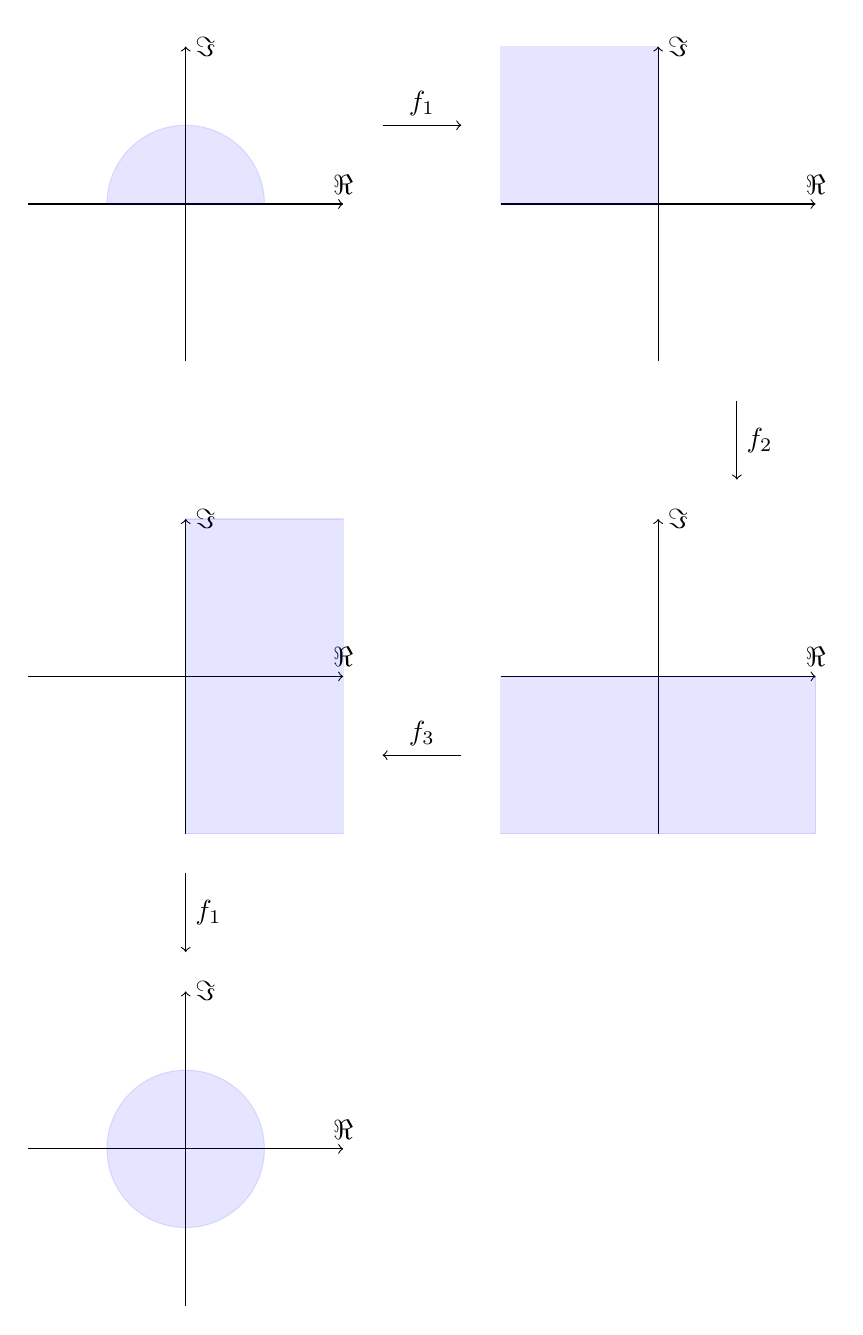
\begin{tikzpicture}[scale=1]
        \tikzset{region/.style={fill, color=blue, opacity=0.1}}
        \begin{scope}[shift={(0, 0)}]
            \draw [->] (-2, 0) -- (2, 0) node[above] {$\Re$};
            \draw [->] (0, -2) -- (0, 2) node[right] {$\Im$};

            \draw[region] (1, 0) arc[start angle=0, end angle=180, radius=1] -- cycle;
        \end{scope}
        \draw[->] (2.5, 1) -- (3.5, 1) node[pos=0.5, anchor=south] {$f_1$};
        \begin{scope}[shift={(6, 0)}]
            \draw [->] (-2, 0) -- (2, 0) node[above] {$\Re$};
            \draw [->] (0, -2) -- (0, 2) node[right] {$\Im$};

            \draw [region] (-2, 0) -- (0, 0) -- (0, 2) -- (-2, 2) -- cycle;
        \end{scope}
        \draw[->] (7, -2.5) -- (7, -3.5) node[pos=0.5, anchor=west] {$f_2$};
        \begin{scope}[shift={(6, -6)}]
            \draw [->] (-2, 0) -- (2, 0) node[above] {$\Re$};
            \draw [->] (0, -2) -- (0, 2) node[right] {$\Im$};

            \draw [region] (-2,0) -- (2, 0) -- (2, -2) -- (-2, -2) -- cycle;
        \end{scope}
        \draw[->] (3.5, -7) -- (2.5, -7) node[pos=0.5, anchor=south] {$f_3$};
        \begin{scope}[shift={(0, -6)}]
            \draw [->] (-2, 0) -- (2, 0) node[above] {$\Re$};
            \draw [->] (0, -2) -- (0, 2) node[right] {$\Im$};

            \draw [region] (0, 2) -- (2, 2) -- (2, -2) -- (0, -2) -- cycle;
        \end{scope}
        \draw [->] (0, -8.5) -- (0, -9.5) node[pos=0.5, anchor=west] {$f_1$};
        \begin{scope}[shift={(0, -12)}]
            \draw [->] (-2, 0) -- (2, 0) node[above] {$\Re$};
            \draw [->] (0, -2) -- (0, 2) node[right] {$\Im$};

            \draw[region] (0, 0) circle[radius=1];
        \end{scope}
    \end{tikzpicture}
    \caption{Diagram of a composition of conformal maps}
    \label{figConfMapsCompose}
\end{figure}
\end{document}